\documentclass[../statistical_learning_notes.tex]{subfiles}
\begin{document}
    %%%%%%%%%%%%%%%%%%%%%%%%%%%%%%%%%%%%%%%%%%%%%%%%%%%%%%%%%%%%%%%%%%%%%%%%%%%%%%%
    \chapter{Linear Model Selection and Regularization}
    Linear models are often simple and easy to interpret at the cost of having high bias if the relationship in the data is not linear. Some considerations about linear models
    \begin{itemize}
        \item If $n >> p$, least square estimates often have less variance. If $n$ is larger than $p$, then least square estimates can have some variance. While if $n < p$, we are looking at non unique solutions which can cause lot of variation in the test predictions.
        \item It is often the case that many of the predictors do not have a relationship with the response. Hence, it is a good idea to remove those and make the model more interpretable at the cost of some bias. Least square estimates almost never give zero coefficients.
    \end{itemize}

    There are major ways in which the number of variables in the model can be reduced
    \begin{itemize}
        \item Selecting a \textbf{subset of variables} that go well with the response. This itself can be done by forward selection, backward elimination etc.
        \item \textbf{Shrinking} some of the \textbf{coefficients} to zero. This is a great help in reducing the variance of the predictions.
        \item \textbf{Dimension Reduction} helps in projecting the $p$ predictors onto a $M$ dimensional space where $M < p$. This utilizes linear combinations to create a set of new features.
    \end{itemize}

    %%%%%%%%%%%%%%%%%%%%%%%%%%%%%%%%%%%%%%%%%%%%%%%%%%%%%%%
    \section{Subset Selection}
    %%%%%%%%%%%%%%%%%%%%%%%%%%%%%%%%%%%
    \subsection{Best Subset Selection}
    This is a naive approach that essentially tries to find the best model among $2^{p}$ models that are trained on all possible subsets of the $p$ variables. As we increase the subset of variables, the training error will monotonically decrease whereas the same cannot be said for the test error. A number of criteria like test MSE, $R^{2}$, AIC etc can be used to pick the models.\newline

    In case of classification models, similar argument holds and a more general error metric $deviance$ can be used. $Deviance$ is defined as $-2 * \log likelihood$ of the data. The smaller the $deviance$, the better the model fit.\newline

    The huge search space presented by this approach easily overfits as the search space presents more opportunities to find better fits. However, this causes a higher variance in the predictions on future data and can possibly also have higher test error.

    
    %%%%%%%%%%%%%%%%%%%%%%%%%%%%%%%%%%%
    \subsection{Forward Stepwise Selection}
    This is a greedy approach that significantly shrinks the search space being checked (in comparison to the best subset selection approach).

    Forward Stepwise Selection Algorithm
    \begin{enumerate}
        \item Let $M_{0}$ denote the null model, i.e., the model with no predictors
        \item For $k = 0, 1, \ldots, p - 1$
        \begin{enumerate}
            \item Consider all $p - k$ models formed by adding a single predictor to the model $M_{k}$
            \item Select the best model $M_{k+1}$ among the $p - k$ models on the basis of the error metric
        \end{enumerate}
        \item From the models $M_{0}, M_{1}, \ldots, M_{p}$, select the one with the lowest cross validation error on the evaluation choosing the appropriate error metric
    \end{enumerate}

    This approach effectively has reduced the search space from $2^{p}$ to $1 + p(p+1)/2$. Although, now it is not guaranteed that the model selected will be the best one among $2^{p}$.


    %%%%%%%%%%%%%%%%%%%%%%%%%%%%%%%%%%%
    \subsection{Backward Stepwise Selection}
    This approach is the opposite of forward stepwise selection. We recursively reduce the number of variables in our model.

    \begin{enumerate}
        \item Let $M_{p}$ denote the complete model, i.e., the model with all p predictors
        \item For $k = p, p-1, \ldots, 1$
        \begin{enumerate}
            \item Consider all $k-1$ models that keep all but one predictors in the current model $M_{k}$
            \item Among these, select the best model $M_{k-1}$ with the lowest error
        \end{enumerate}
        \item From the models $M_{0}, M_{1}, \ldots, M_{p}$, select the one with the lowest cross validation error on the evaluation choosing the appropriate error metric 
    \end{enumerate}

    The number of models explored is same as the forward stepwise method.\newline
    A hybrid approach is usually selected where we start with the usual forward selection method, but while adding variables, we do not add a variable if it does not give significant improvement. Another approach can be to remove redundant variables using p-test at every step of forward selection.

    
    %%%%%%%%%%%%%%%%%%%%%%%%%%%%%%%%%%%
    \section{Metrics for evaluating Subset Models}
    In linear models, as we add more variables, the training error usually monotonically decreases. Test error may not behave in the same way. When training a model, the coefficients obtained are specific for minimizing the training error and hence will have less bias in comparison to the test error. \newline
    Hence, subset evaluation using training error will usually favour models with more number of variables. To overcome this
    \begin{itemize}
        \item Correct the training error estimate to correctly calculate test error
        \item Use a validation test or $k$-fold validation for better estimate of test error
    \end{itemize}
    
    %%%%%%%%%%%%%%%%%%%%%%%%%%%%%%%%%%%
    \subsection{$C_{p}$ Estimate}
    For a least square fitted model,
    \begin{align*}
        C_{p} = \frac{1}{n}(RSS + 2p\hat{\sigma}^{2})
    \end{align*}
    $p$ is the number of predictors and $\hat{\sigma}^{2}$ is the estimate of the error associated with each observation. This is typically evaluated using the model built on all $p$ predictors.\newline
    Clearly, as $p$ increases, we are penalizing the model more to compensate for the decrease in the training RSS. When $\hat{\sigma}$ is an unbiased estimate of $\sigma$, we can show that this is infact an unbiased estimate of the test MSE.


    %%%%%%%%%%%%%%%%%%%%%%%%%%%%%%%%%%%
    \subsection{Akaike Information Criterion (AIC)}
    AIC is defined for a large class of models fit by the maximum likelihood estimate.\newline
    For least squares fit in linear models, the errors are assumed to be gaussian and thus, AIC and least squares mean the same thing. For this case
    \begin{align*}
        AIC = \frac{1}{n\hat{\sigma}^2}(RSS + 2p\hat{\sigma}^2)
    \end{align*}
    where we have omitted an additive constant for the sake of simplicity.\newline
    For least squares models, $C_{p}$ and AIC are proportional to each other.


    %%%%%%%%%%%%%%%%%%%%%%%%%%%%%%%%%%%
    \subsection{Bayesian Information Criterion (BIC)}
    BIC is derived from a Bayesian point of view, but ends up looking similar to the above defined errors.\newline
    For least squares error without constants, the BIC is
    \begin{align*}
        BIC = \frac{1}{n\hat{\sigma}^{2}} (RSS + \log(n)p\hat{\sigma}^{2})
    \end{align*}
    Note that the $\log(n)$ term will put a heavier weight on the error term for large $p$. Hence, BIC will tend to select models with lower number of variables in comparison to say $C_{p}$.

    
    %%%%%%%%%%%%%%%%%%%%%%%%%%%%%%%%%%%
    \subsection{Adjusted $R^{2}$}
    Recall that $R^{2}$ is defined as $1 - RSS/TSS$. Adjusted $R^{2}$ is
    \begin{align*}
        Adjusted\;R^{2} = 1 - \frac{\frac{RSS}{n-p-1}}{\frac{TSS}{n-1}}
    \end{align*}
    This adjusted $R^{2}$ might increase or decrease when adding variables due to the terms corresponding to $p$. The intuition is that, after the correct number of variables have been identified, the decrease in RSS is less in comparison to the decrease in $n-p-1$ which will slightly increase the Adjusted $R^{2}$.


    %%%%%%%%%%%%%%%%%%%%%%%%%%%%%%%%%%%%%%%%%%%%%%%%%%%%%%%
    \section{Shrinkage Methods}
    Instead of using a subset of predictors, we can also use all of the predictors and shrink the coefficients towards zero. This approach significantly reduces the variance in the model estimates. The famous ones here are \emph{Ridge Regression} and \emph{Lasso Regression}.

    
    %%%%%%%%%%%%%%%%%%%%%%%%%%%%%%%%%%%
    \subsection{Ridge Regression}
    Ridge Regression is very similar to the least square estimate for linear regression except that we add a term corresponding to the squared sum of the regression coefficients in the error.
    \begin{align*}
        error &= RSS + \lambda \sum_{j=1}{p}\beta_{j}^{2}\\
              &= (Y-X\beta)^{T}(Y-X\beta) + \lambda \beta^{T}\beta
    \end{align*}
    $\lambda$ is a tuning parameter that needs to be chosen separately. It acts as a weight between the error in the data and how large are the regression coefficients. It is also known as the shrinkage penalty.\newline
    Note that we will not include the intercept term in shrinkage because it is simply the mean estimate of the model when all the predictors are zero and may not necessarily zero.\newline

    Using least squares estimate,
    \begin{align*}
        error &= (Y-X\beta)^{T}(Y-X\beta) + \lambda \beta^{T}\beta\\
        \frac{\partial error}{\partial \beta} &= 0\\
        \implies 0 &= -Y^{T}X - Y^{T}X + \beta^{T}X^{T}X + \beta^{T}X^{T}X + \lambda \beta^{T} + \lambda \beta^{T}\\
        \beta^{T}(X^{T}X + \lambda I) &= Y^{T}X\\
        (X^{T}X + \lambda I)^{T}\beta &= X^{T}Y\\
        (X^{T}X + \lambda I)\beta &= X^{T}Y\\
        \Aboxed{\beta &= (X^{T}X + \lambda I)^{-1}X^{T}Y}  
    \end{align*}
    $\lambda = 0$ will result in the simple least squares regression while $\lambda \to \inf$ will force the coefficients to go towards zero.\newline

    As is clear from the formula, the error term is sensitive to the actual scale of the coefficients which is ultimately dependent on the predictors themselves. In a simple least squares regression, the coefficients will scale up and down depending on how the data is scaled. The same is not true for Ridge Regression.\newline
    Hence when using \textbf{Ridge Regression, it is always advisable to \emph{standardize} the predictors} before training the model using
    \begin{align*}
        \tilde{x}_{ij} = \frac{x_{ij}}{\sqrt{\frac{1}{n}\sum_{i=1}{n}(x_{ij}-\bar{x}_{j})^{2}}}
    \end{align*}

    The success of Ridge Regression is based in the \textbf{bias variance tradeoff}. If the data is linear, simple linear regression will have a very low bias but high variance, making it sensitive to the training data. As $\lambda$ is introduced, it forces the model to have less flexibility by reducing the coefficiets value and subsequently their power on the prediction. This causes a reduction in the variance at expense of slight increase in bias. However, this trend is not monotonic with increasing $\lambda$ and the appropriate value must be chosen based on the errors observed.\newline
    \textbf{Ridge regression will tend to give similar coefficient values for correlated variables.} 

    
    %%%%%%%%%%%%%%%%%%%%%%%%%%%%%%%%%%%
    \subsection{Lasso Regression}
    Notice that Ridge Regression will try to reduce the value of some of the coefficients, but it will never set them to exactly zero. Hence, we will end up using all the $p$ predictors in the model which may not be interpretable if the value of $p$ is large.\newline

    Lasso Regression comes over this disadvantage by defining the error as
    \begin{align*}
        error &= RSS + \lambda \sum_{j=1}^{p}\mid \lambda_{j} \mid
    \end{align*}

    When \textbf{$\lambda$ is sufficiently large, Lasso Regression forces some of the variables to be exactly zero}. This is very useful in reducing the subset of variables that we use in the model, thereby increasing model interpretability.\newline
    \textbf{Lasso Regression can give different coefficient values to correlated variables.}


    %%%%%%%%%%%%%%%%%%%%%%%%%%%%%%%%%%%
    \subsection{Alternative Formulation to Ridge and Lasso Regression}
    These regressions can also be considered as solving a constrained optimisation problem
    \begin{align*}
        &\minimize_{\beta}  \bigg\{\sum_{i=1}^{n} (y_{i} - \beta_{0} - \sum_{j=1}^{p}\beta_{j}x_{ij})^{2} \bigg\} \text{\;\;\;subject to\;} &&\sum_{j=1}^{p}\beta_{j}^{2} \leq s \\
        &\minimize_{\beta}  \bigg\{\sum_{i=1}^{n} (y_{i} - \beta_{0} - \sum_{j=1}^{p}\beta_{j}x_{ij})^{2} \bigg\} \text{\;\;\;subject to\;} &&\sum_{j=1}^{p}\mid \beta_{j} \mid \leq s
    \end{align*}
    for Ridge and Lasso regression respectively. This holds true because these regressions are effectively trying to limit the size of the coefficients themselves. For $\lambda = 0$, we have no bound on the size and $s$ in equations above is close to $\inf$. As $\lambda$ increases, $s$ will start to decrease and be $0$ for $\lambda \to \inf$. \newline

    The equations above can be interpreted as finding the minimum RSS among the points that lie inside the geometric shapes defined by the constraints. For $p = 2$, Ridge defines a circle $\beta_{1}^{2} + \beta_{2}^{2} \leq s$ and Lasso defines a diamond $\mid \beta_{1} \mid + \mid \beta_{2} \mid \leq s$.

    
    %%%%%%%%%%%%%%%%%%%%%%%%%%%%%%%%%%%
    \subsection{Variable Selection Property of Lasso Regression}
    \begin{figure}[h]
    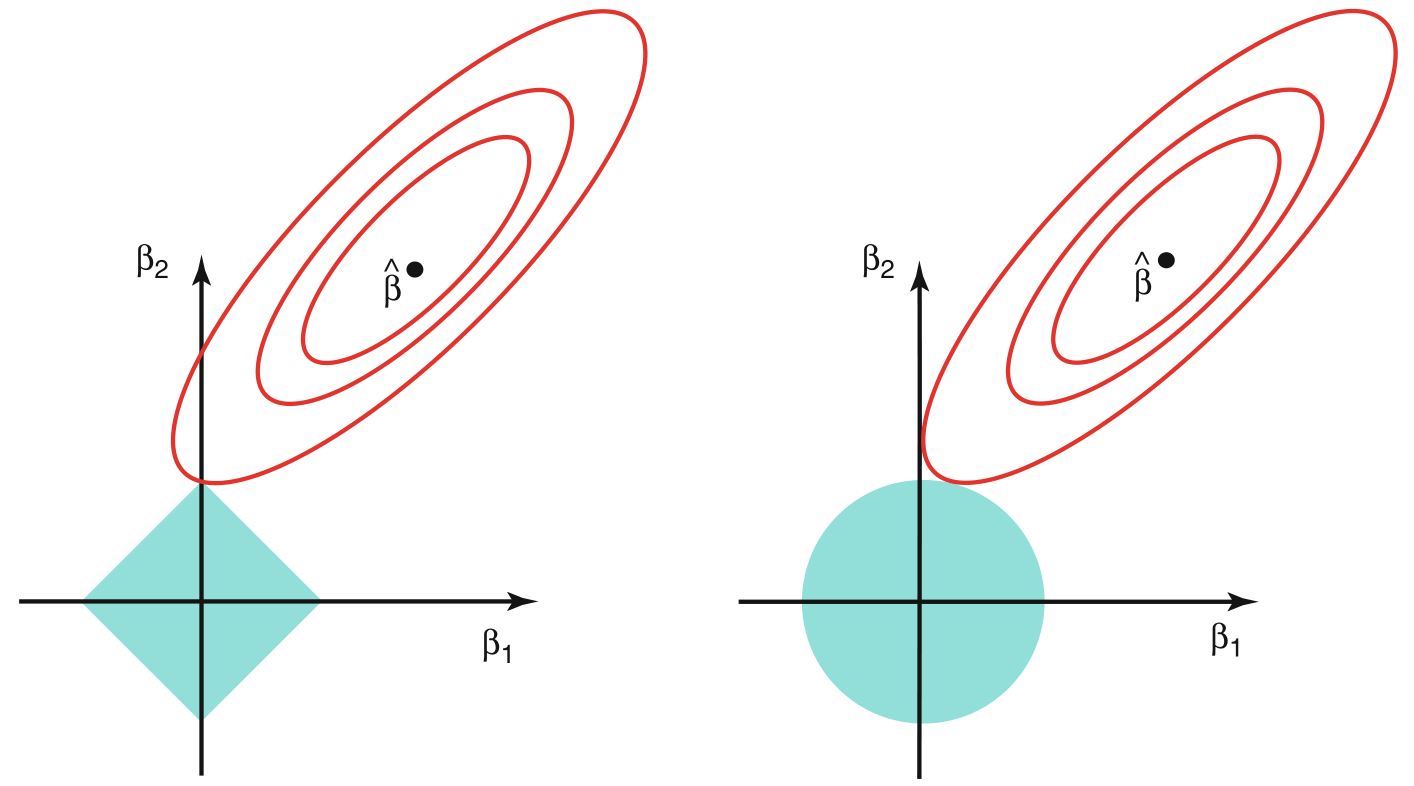
\includegraphics[scale=0.4]{lasso_contours}
    \centering
    \caption{For $p=2$, the left and right images correspond to Lasso and Ridge Regression.}
    \label{fig:lasso_contour} %\ref{fig:lasso_contour}
    \end{figure}

    In the figure \ref{fig:lasso_contour}, $\hat{\beta}$ corresponds to the least squares estimate of $\beta$ and the contours in red colour show the same value of RSS. The blue coloured regions correspond to the constraints defined above (diamond for lasso and circle for ridge).\newline
    Clearly, circle being a smooth shape, the lowest RSS contour will not usually touch it at one of the axis points. However, for the sharp diamond shape, the least RSS value is likely to be encountered along the axis. The shapes of the constraint regions can be controlled through $\lambda$ and for lasso, more constrained models (small $s$ or higher $\lambda$) will cause more of the coefficients to be zero. The argmuents are very well valid in higher dimensions as well.

    
    %%%%%%%%%%%%%%%%%%%%%%%%%%%%%%%%%%%
    \subsection{Bayesian Interpretation}
    Lasso and Ridge Regression are also natural solutions when the the coefficients are assumed to have certain specific priors.\newline
    \begin{figure}[h]
        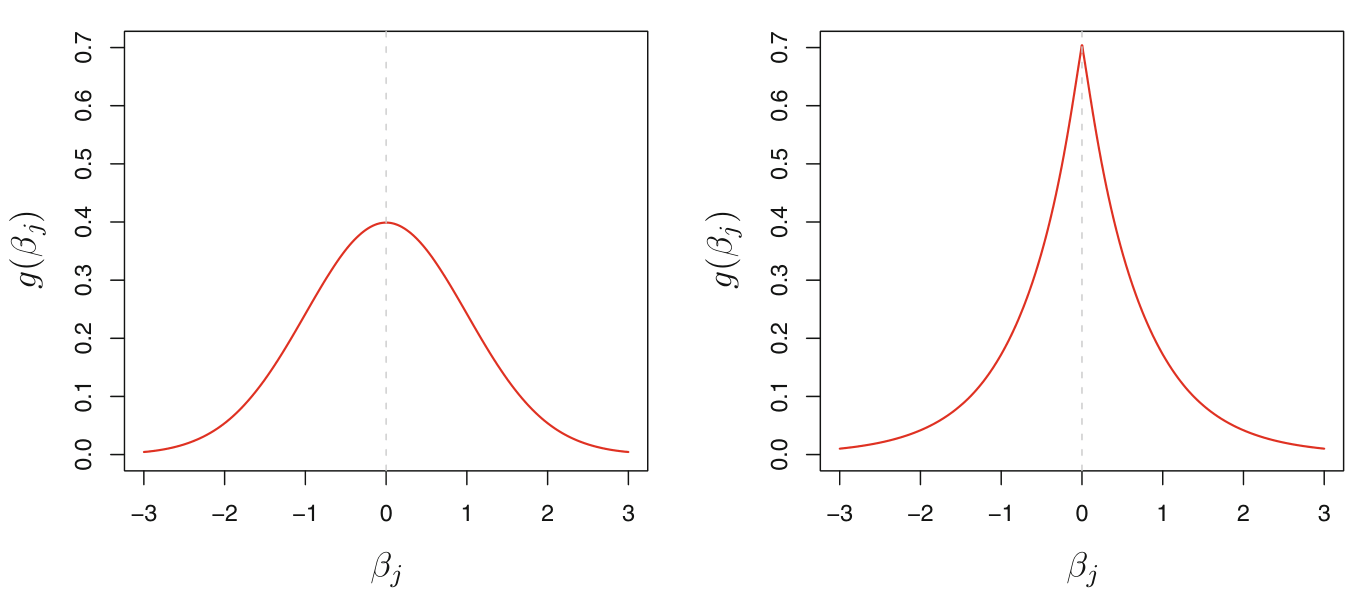
\includegraphics[scale=0.4]{lasso_bayes}
        \centering
        \caption {Gaussian prior on left and double exponential on the right}
        \label{fig:lasso_bayes}
    \end{figure}
    
    \begin{align*}
        p(\beta|X,Y) &\propto f(Y|X,\beta)p(\beta|X) = f(Y|X,\beta)p(\beta) \tag*{assuming X is constant}\\
        Y &= \beta_{0} + \beta_{1}X_{1} + \cdots + \beta_{p}X_{p} + \epsilon\\
        \text{Assume, } p(\beta) &= \prod_{j=1}^{p} \beta_{p} \tag*{for some density function $g$}  
    \end{align*}

    The following are observed for different priors on $\beta$

    \begin{itemize}
        \item When the density function of $\beta_{j}$ is assumed to be a standard normal, the posterior is same as solving the ridge regression error function
        \item When the density function is assumed to be a double exponential, the posterior is the same as solving lasso error function
    \end{itemize}

    From the visuals of the priors in figure \ref{fig:lasso_bayes}, double exponential is steeply peaked at zero, which clearly implies that the prior itself assumes some of the coefficients are likely zero. On the other hand, the gaussian priod is flatter and does not necessarily require the coefficients to be zero.


    %%%%%%%%%%%%%%%%%%%%%%%%%%%%%%%%%%%%%%%%%%%%%%%%%%%%%%%
    \section{Dimension Reduction Methods}
    The methods seen above achieve reduction in variance by either reducing the number of variables being used for estimation, or reduce the value of coefficients of those variables.\newline
    Dimensionality reduction uses a \textbf{linear map} to convert the original $p$ variables to $M$ variables where $M < p$.
    \begin{align*}
        Z_{m} &= \sum_{j=1}^{p} \phi_{jm}X_{j} \tag*{where $\phi_{jm}$ are constants} \\
        RSS &= \sum_{i=1}^{n} (y_{i} - (\theta_{0}+\sum_{m=1}^{M}\theta_{m}Z_{m}))^{2} \tag*{where $\theta_{m}$ are linear regression coefficients for $Z_{m}$}
    \end{align*}
    This new formulation restructures the original least squares formula. The whole process now is
    \begin{itemize}
        \item Obtain the linear map using techniques like PCA
        \item Use least squares on the transformed predictors to obtain regression estimates
    \end{itemize}


    %%%%%%%%%%%%%%%%%%%%%%%%%%%%%%%%%%%
    \subsection{Principal Components Analysis (PCA)}
    PCA is one of the most common methods used for dimensionality reduction. It is based on the principle of finding those directions that \textbf{maximize the variance of data}. The intuition behind finding this direction is that this separates the data best given the high variance. Hence, the performance of a classifier/regressor would be better if the training was done using the transformed predictors. \newline

    Assume that we want to find $M$ components for PCA, where $M <= p$. Then,
    \begin{enumerate}
        \item Find the direction/projection of the data that gives the maximum variance under the constraint $\sum_{j=1}^{p}\phi_{jm}^{2} = 1$ (normalized vector) for obtaining the $m^{th}$ transformed predictor
        \item If the total components found is $< M$, repeat step 1 with the added constraint that the next component has zero correlation with the previous component
    \end{enumerate}
    This constraint of finding components with zero correlation essentially means that in the multidimensional space, we are finding a set of \textbf{orthogonal vectors}. The order of choosing the new predictors is in decreasing order of the information they contain. Thus, the first predictor will now containt the most information. \newline

    %%%%%%%%%%%%%%%
    \paragraph{Derivation of PCA}
    It is a good idea to \textbf{standardize the variables before running PCA}. Not only is it easier to derive the components, but they are also unaffected by the scale of the individual variables (since we know that scaling a variable multiplies the variance by square of the scaler and PCA is all about finding maximum variances !). \newline \newline
    After setting the the mean of all predictors to zero and standard deviation to one, the components can be derived by considering the following optimization problem
    \begin{gather*}
        \maximize_{\phi_{11},\ldots,\phi_{p1}} \big\{ \frac{1}{n} \sum_{i=1}^{n} (\sum_{j=1}^{p}\phi_{j1}x_{ij})^{2} \big\} \text{ subject to } \sum_{j=1}^{p} \phi_{j1}^{2} = 1\\
        \text{Or, } \maximize_{\Phi_{1}} \frac{1}{n} Z_{1}^{T}Z_{1} \text{ subject to } \sum_{j=1}^{p} \phi_{j1}^{2} = 1\\
        \text{Where } Z_{1} = X\Phi_{1}\\
        \text{Define the Lagrangian } L(\Phi_{1}, \lambda) = \frac{1}{n} (\Phi_{1}^{T}X^{T}X\Phi_{1}) - \lambda (\Phi^{T}\Phi - 1)\\
        \frac{\partial L(\Phi_{1}, \lambda)}{\partial \lambda} = 0 \text{, and } \frac{\partial L(\Phi_{1}, \lambda)}{\partial \Phi_{1}} = 0 \\
        \text{Giving, } 2\frac{1}{n}(\Phi_{1}^{T}X^{T}X) - 2\lambda \Phi_{1}^{T} = 0 \text{ and } \Phi_{1}^{T}\Phi_{1} - 1 = 0\\
        \frac{X^{T}X}{n}\Phi_{1} = \lambda \Phi_{1}\\
        \text{Since all } X_{i} \text{ are centered, } \frac{X^{T}X}{n} \text{ is the covariance matrix } \Sigma_{X}\\
        \Sigma_{X} \Phi_{1} = \lambda \Phi_{1} \text{ with } \Phi_{1}^{T}\Phi_{1} = 1\\
    \end{gather*}
    Which is nothing but the \textbf{Eigenvectors of the Covariance Matrix of $X$}. Notice that the maximization is achieved through the eigenvector with the highest eigenvalue. Since $\Sigma_{X}$ is positive semi-definite, all the eigenvalues will be $\geq 0$. \newline
    Furthermore, we know that all eigenvectors are orthogonal to each other, and hence they will also satisfy the condition that all the linear mapping vectors are not correlated to each other. \newline
    If we try to find the coefficients for $Z_{2}$, we are looking at the exact same optimization, but with the additional constraint that $\Phi_{2}$ is not correlated to $\Phi_{1}$. This will yield the second eigenvector of the covariance matrix. \newline
    Hence, \textbf{the linear maps for obtaining the PCA transformations are nothing but the eigenvectors of the covariance matrix $\Sigma_{X}$ of the original data $X$}. We have a total of $p$ eigenvectors and thus, the maximum components obtainable is also $p$.

    %%%%%%%%%%%%%%%
    \paragraph{Explained Variance}
    The variance explained by the $m^{th}$ component is nothing but the ratio of variance of $Z_{m}$ and total variance of the data. Mathematically this is
    \begin{align*}
        \text{Explained variance of component } m &= \frac{\frac{1}{n}\sum_{i=1}^{n} (\sum_{j=1}^{p} \phi_{jm} x_{ij})}{\frac{1}{n}\sum_{i=1}{n} \sum_{j=1}{p} x_{ij}^2}\\
                &= \frac{\frac{1}{n}Z_{m}^{T}Z_{m}}{tr(\frac{X^{T}X}{n})}\\
                &= \frac{\Phi_{m}^{T}\frac{X^{T}X}{n}\Phi_{m}}{tr(\Sigma_{X})}\\
    \end{align*}
    However, note that in the derivation, $\Phi_{m}$ is the eigenvector and thus, $(X^{T}X)\Phi_{m} = \lambda_{m}\Phi_{m}$ and $\Phi_{m}^{T}\Phi_{m} = 1$. Substituiting in the above equation,
    \begin{align*}
        \text{Explained variance } &= \frac{\lambda_{m}}{tr(\Sigma_{X})}\\
        \text{or, } \Aboxed{\text{Explained variance } &= \frac{\lambda_{m}}{\lambda_{1} + \cdots +\lambda_{p}}}
    \end{align*}
    Where the last equation comes from the fact that the trace of a matrix is simply the sum of it's eigenvalues.\newline
    A \textbf{Scree Plot} is a plot between the explained variance and the index of the prinicple components. It's cumulative version can be used to determine the number of components to keep on the basis of how much of the total variance we want to explain. The elbow point of the Scree Plot can also help determine the components at which the explained variance drops significantly.
    \paragraph{Principal Components Regression (PCR)}
    is simply using some $m$ out of $M$ components to perform linear regression. This approach will typically work best when a few components of the PCA sufficiently explain the whole data. This way we reduce the variance at the cost of slight change in bias. PCR can also be viewed as a continuous version of Ridge Regression.
    

    %%%%%%%%%%%%%%%%%%%%%%%%%%%%%%%%%%%
    \subsection{Partial Least Squares}
    This method is closely related to PCA/PCR. In the previous methods, an unsupervised approach was used to project the matrix $M$ onto a lower dimensional space. This transformation did not take $Y$, the response, into consideration. PLS will incorporate $Y$ as well for finding the transformations.\newline
    The algorithm is as follows
    \begin{enumerate}
        \item Calculate the coefficients for the first component as the coefficient obtained by regressing $Y$ on $X_{j}$
        \item Using this component, regress $X_{j}$'s on $Z_{1}$ and get the residuals. These are the unexplained components of the variables.
        \item Calculate $Z_{2}$ using $Y$ and these residuals
        \item Repeate the process above till $M$ components are obtained
    \end{enumerate}

    Though this procedure looks slightly more involved, it performs not better than lasso regression and PCR in practice. Although this method reduces bias, it also leads to quite an increase in variance as well, making the method not very useful.

    %%%%%%%%%%%%%%%%%%%%%%%%%%%%%%%%%%%%%%%%%%%%%%%%%%%%%%%
    \section{Curse of Dimensionality}
    Most of the methods discuss here \textbf{work well when $n >> p$}. There can be many reasons why the model may not perform well in higher dimensions, but the major one will be the fact that as more and more dimensions are added to the model, chances of overfitting increase and so do the chances that the additional variables are simply noise.\newline
    We refer to the problem of training a model a high dimensional problem when $p > n$, or we have more data than number of predictors. Note that it is easy to obtain $R^{2} = 1$ in such a setting which consequently leads to $\hat{\sigma}^{2} \approx 0$. Metrics like $C_{p}$, AIC, BIC become useless.\newline
    Hence, in higher dimensional settings, it is important to obtain model performance on unseen data as there is a good chance of obtaining perfect results on the training set. Metrics associated with the training set can thus prove to be misleading.

    \paragraph{Intuition}
    for the curse of dimensionality can be easily obtained in the context of KNN.\newline
    Suppose the data is uniformly distributed along any dimension considered. Let the model be built in such a way that when making predictions, it uses $10\%$ of the data along all dimensions. \newline
    In the case of a single dimension, we need $10\%$ of the data. In the case of 10 dimensions, we will need to check $10\% ^{10} = 10^{-8}\%$ of data. Clearly this number grows as we consider more and more dimensions.\newline
    Thus, as the number of dimensions grow, we require substantially more data as the data observable in the neighborhood of the point is extremely small. This illustrates the fact that in higher dimensions, having less data will lead to a poor model.


    
    %%%%%%%%%%%%%%%%%%%%%%%%%%%%%%%%%%%%%%%%%%%%%%%%%%%%%%%
    \section{Exercises}
    \begin{enumerate}
        %%%%%Q1
        \item We perform the best subset, forward stepwise and backward stepwise on a single data set and obtain p+1 models containing $0, 1, \ldots, p$ predictors.
        \begin{enumerate}
            \item Which of the three models with $k$ predictors has the smalles training RSS ?
            \item Which of the three models with $k$ predictors has the smallest test RSS ?
            \item True or False
            \begin{enumerate}
                \item The predictors in the $k$-variable model identified by forward stepwise are a subset of the predictors in the $(k+1)$-variable model identified by forward stepwise selection.
                \item The predictors in the $k$-variable model identified by backward stepwise are a subset of the predictors in the $(k+1)$-variable model identified by backward stepwise selection.
                \item The predictors in the $k$-variable model identified by backward stepwise are a subset of the predictors in the $(k + 1)$-variable model identified by forward stepwise selection.
                \item The predictors in the $k$-variable model identified by forward stepwise are a subset of the predictors in the $(k+1)$-variable model identified by backward stepwise selection.
                \item The predictors in the $k$-variable model identified by best subset are a subset of the predictors in the $(k + 1)$-variable model identified by best subset selection.
            \end{enumerate}
        \end{enumerate}

        %%%%%Q2
        \item For parts (a) through (c), indicate the correct choice and explain the answer.
        \begin{enumerate}
            \item The lasso, relative to least square is
            \begin{enumerate}
                \item More flexible and hence will give improved prediction accuracy when its increase in bias is less than its decrese in variance.
                \item More flexible and hence will give improved prediction accuracy when its increase in variance is less than its decrease in bias.
                \item Less flexible and hence will give improved prediction accuracy when its increase in bias is less than its decrease in variance.
                \item Less flexible and hence will give improved prediction accuracy when its increase in variance is less than its decrease in bias.
            \end{enumerate}
            \item Repeat (a) for ridge regression relative to least squares.
            \item Repeat (b) for non-linear methods relative to least squares.
        \end{enumerate}
        
        %%%%%Q3
        \item Suppose we estimate regression coefficients in a linear model by minimizing
        \begin{gather*}
            \sum_{i=1}^{n}\bigg( y_{i} - \beta_{0} - \sum_{j=1}^{p}\beta_{j}x_{ij} \bigg)^{2} \text{ subject to } \sum_{j=1}^{p}\mid \beta_{j} \mid \leq s
        \end{gather*}
        for a particular value of $s$. For the following parts, indicate which of the options is correct and explain.
        \begin{enumerate}
            \item As we increase $s$ from 0, the training RSS will
            \begin{enumerate}
                \item Increase initially, and then eventually start decreasing in an inverted U shape.
                \item Decrease initially, and then eventually start increasing in a U shape.
                \item Steadily increase.
                \item Steadily decrease.
                \item Remain constant.
            \end{enumerate}
            \item Repeat (a) for test RSS.
            \item Repeat (a) for variance.
            \item Repeat (a) for (squared) bias.
            \item Repeat (a) for the irreducible error.
        \end{enumerate}
        
        %%%%%Q4
        \item Suppose we estimate regression coefficients in a linear model by minimizing
        \begin{gather*}
            \sum_{i=1}^{n}\bigg( y_{i} - \beta_{0} - \sum_{j=1}^{p}\beta_{j}x_{ij} \bigg)^{2} + \lambda \sum_{j=1}^{p}\beta_{j}^{2}
        \end{gather*}
        for a particular value of $\lambda$. For the following parts, indicate which of the options is correct and explain.
        \begin{enumerate}
            \item As we increase $s$ from 0, the training RSS will
            \begin{enumerate}
                \item Increase initially, and then eventually start decreasing in an inverted U shape.
                \item Decrease initially, and then eventually start increasing in a U shape.
                \item Steadily increase.
                \item Steadily decrease.
                \item Remain constant.
            \end{enumerate}
            \item Repeat (a) for test RSS.
            \item Repeat (a) for variance.
            \item Repeat (a) for (squared) bias.
            \item Repeat (a) for the irreducible error.
        \end{enumerate}

        %%%%%Q5
        \item It is well-known that ridge regression tends to give similar coefficient values to correlated variables, whereas the lasso may give quite different coefficient values to correlated variables. We will now explore this property in a very simple setting.\newline
        Suppose that $n = 2$, $p = 2$, $x_{11} = x_{12}$, $x_{21} = x_{22}$. Furthermore, suppose that $y_{1} +y_{2} = 0$ and $x_{11} +x_{21} = 0$ and $x_{12} +x_{22} = 0$, so that the estimate for the intercept in a least squares, ridge regression, or lasso model is zero: $\hat{\beta_{0}} = 0$.
        \begin{enumerate}
        \item Write out the ridge regression optimization problem in this setting.
        \item Argue that in this setting, the ridge coefficient estimates satisfy $\hat{\beta_{1}} = \hat{\beta_{2}}$.
        \item Write out the lasso optimization problem in this setting.
        \item Argue that in this setting, the lasso coefficients $\hat{\beta_{1}}$ and $\hat{\beta_{1}}$ are not unique—in other words, there are many possible solutions to the optimization problem in (c). Describe these solutions.
        \end{enumerate}
        
        %%%%%Q6
        \item Using the bayesian formulation given below, derive the ridge and lasso formulations
        \begin{align*}
            p(\beta|X,Y) \propto f(Y|\beta,X)p(\beta|X) = f(Y|\beta,X)p(\beta)
        \end{align*}
        \begin{enumerate}
            \item Suppose $y_{i} = \beta_{0} + x_{i}^{T}\beta + \epsilon_{i}$ where $\epsilon_{i}$ is normal with mean $0$ and variance $\sigma^{2}$. Calculate the likelihood of the data.
            \item Assume the following prior for $\beta$: $\beta_{1},\ldots,\beta_{p}$ are independent identically distributed with the distribution $p(\beta) = \frac{1}{2b}\exp(-\mid \beta \mid/b)$. Write the posterior for $b$ in this setting.
            \item Argue that the lasso estimate is the \emph{mode} of the posterior on $\beta$.
            \item Now assume that the $\beta$ are independently and identically distributed with the mean $0$ and variance $c$. Find the posterior of the $\beta$ in this case.
            \item Argue that the ridge regression estimate is both the mode and mean for $\beta$ under this distribution.
        \end{enumerate}
    \end{enumerate}

    \textbf{Answers}
    \newline
    \begin{enumerate}
        %%%%%Q1
        \item
        \begin{enumerate}
            \item Best subset model will have the lowest training RSS as it looks over all possible subsets of models.
            \item Best subset model will typically overfit and thus forward or backward stepwise models will have lower test RSS.
            \item
            \begin{enumerate}
                \item True as we add variables to the last model.
                \item True as we remove variables from the last model.
                \item False as this is not necessary. The paths chosen are independent.
                \item False.
                \item False as the set of variables can be completely independent.
            \end{enumerate}
        \end{enumerate}

        %%%%%Q2
        \item
        \begin{enumerate}
            \item iii as lasso is less flexible (some coefficients are zero) which decreases variance with an increase in bias.
            \item iii as it is similar to lasso in terms of purpose of use.
            \item ii as non-linear models make less assumptions and are more flexible. This reduces bias at expense of variance.
        \end{enumerate}
        
        %%%%%Q3
        \item
        \begin{enumerate}
            \item Refer to \ref{fig:lasso_contour}. As we increase s, we are expanding the region of allowed $\beta$. Hence, we are moving closer to the least squares fit which gives minimum training RSS.
            \item We have high bias with a constant model. As $s$ increases, the test RSS initially decreases and then begins into increase as we keep relaxing the model, giving a U shape.
            \item Constant model has zero variance. It increases as we relax the model (increase $s$).
            \item By bias variance tradeoff, bias reduces as $s$ increases.
            \item It is always constant.
        \end{enumerate}

        %%%%%Q4
        \item
        \begin{enumerate}
            \item As $\lambda$ increases, the model becomes more constrained and training RSS increases.
            \item At $\lambda$ the model has minimum training RSS and high test RSS. As $\lambda$ increases, test RSS initially decreases until it is high for large $\lambda$.
            \item As the model becomes less and less flexible to a constant model, the variance keeps decreasing.
            \item By bias variance tradeoff, bias will keep increasing (it's minimum for least squares fit).
            \item By definition, it remains constant.
        \end{enumerate}
        
        %%%%%Q5
        \item
        \begin{enumerate}
            \item The data points after substituitions become $((x_{11}, x_{11}), y_{1})$ and $((-x_{11}, -x_{11}), -y_{1})$. The optimization functhion then becomes
            \begin{align*}
                RSS &= \sum_{i=1}^{n}(y_{i} - \sum_{j=1}^{p} \beta_{j}x_{ij})^{2} + \lambda \sum_{j=1}^{p}\beta_{j}^{2}\\
                  &= 2(y_{1}-x_{11}(\beta_{1}+\beta_{2}))^{2} + \lambda(\beta_{1}^{2} + \beta_{1}^{2})
            \end{align*}
            \item Taking partial derivates with $\beta_{1}$ and $\beta_{2}$,
            \begin{align*}
                4(y_{1} - x_{11}(\beta_{1} + \beta_{2}))(-x_{11}) + 2\lambda \beta_{1} &= 0\\
                4(y_{1} - x_{11}(\beta_{1} + \beta_{2}))(-x_{11}) + 2\lambda \beta_{2} &= 0
            \end{align*}
            which gives $\beta_{1} = \beta_{2}$.
            \item In a similar fashion to above, the final optimization is
            \begin{align*}
                 RSS = 2(y_{1}-x_{11}(\beta_{1}+\beta_{2}))^{2} + \lambda(\mid \beta_{1} \mid + \mid \beta_{1} \mid)
            \end{align*}
            \item Taking partial derivates with $\beta_{1}$ and $\beta_{2}$,
            \begin{align*}
                4(y_{1} - x_{11}(\beta_{1} + \beta_{2}))(-x_{11}) + 2\lambda \frac{\mid \beta_{1} \mid}{\beta_{1}} &= 0\\
                4(y_{1} - x_{11}(\beta_{1} + \beta_{2}))(-x_{11}) + 2\lambda \frac{\mid \beta_{2} \mid}{\beta_{2}} &= 0
            \end{align*}
            which gives $\frac{\mid \beta_{1} \mid}{\beta_{1}} = \frac{\mid \beta_{2} \mid}{\beta_{2}}$, clearly not a unique solution.
        \end{enumerate}
        
        %%%%%Q6
        \item
        \begin{enumerate}
            \item For any $y_{i}$, the distribution given $X$ and $\beta$ is normal since $y_{i}$ = constant + Normal. The constant is $\beta_{0} + x_{i}\beta$ and the variance is $\sigma^{2}$.
            \begin{align*}
                f(Y|X,\beta) = \prod_{i=1}^{n} \frac{1}{\sqrt{2\pi \sigma^{2}}}\exp(-\frac{(y_{i}-\beta_{0}-x_{i}\beta)^{2}}{2\sigma^{2}})
            \end{align*}
            \item The prior for $\beta$ will simply be the product of all the $\beta_{i}$. The posterior thus becomes
            \begin{align*}
                p(\beta|X,Y) &= f(Y|X,\beta)\prod_{j=1}^{p}\frac{1}{2b}exp{-\frac{\mid \beta_{j} \mid}{b}}\\
                \ln(p(\beta|X,Y)) &= \ln((\frac{1}{\sqrt{2\pi \sigma^{2}}})^{n} (\frac{1}{2b})^{p}) + \sum_{i=1}^{n} -\frac{(y_{i}-\beta_{0}-x_{i}\beta)^{2}}{2\sigma^{2}} + \sum_{j=1}^{p} -\frac{\mid \beta_{j} \mid}{b}
            \end{align*}
            Removing constants and adjusting (includling $-1$), maximizing above equation is same as minimizing
            \begin{align*}
                \sum_{i=1}^{n} (y_{i}-\beta_{0}-x_{i}\beta)^{2} + \frac{2\sigma^{2}}{b}\sum_{j=1}^{p} \mid \beta_{j} \mid
            \end{align*}
            which is the Lasso regression optimization function with $\lambda = 2\sigma^{2}/b$.

            \item $\beta$ obtained as a result of maximizing the posterior $p(\beta|X,Y)$ is the \emph{mode} of that distribution and also happens to be the solution of the lasso regressin optimization function.

            \item The posterior is similar in form to the one derived above with minor changes
            \begin{align*}
                p(\beta|X,Y) &= f(Y|X,\beta)\prod_{j=1}^{p}\frac{1}{2c^{2}}exp{-\frac{\beta_{j}^{2}}{2c^{2}}}\\
                \ln(p(\beta|X,Y)) &= \ln((\frac{1}{\sqrt{2\pi \sigma^{2}}})^{n} (\frac{1}{2c^{2}})^{p}) + \sum_{i=1}^{n} -\frac{(y_{i}-\beta_{0}-x_{i}\beta)^{2}}{2\sigma^{2}} + \sum_{j=1}^{p} -\frac{\beta_{j}^{2}}{2c^{2}}
            \end{align*}
            \item Maximizing the above posterior is same as minimizing
            \begin{align*}
                \sum_{i=1}^{n} (y_{i}-\beta_{0}-x_{i}\beta)^{2} + \frac{2\sigma^{2}}{b}\sum_{j=1}^{p} \beta_{j}^{2}
            \end{align*}
            which is a quadratic. The log of posterior is itself a parabola. The $\beta$ that maximizes the posterior is not only the mode of that distribution, but also the mean (due to the symmetry). And coincidentally, it will also minimize the ridge regression optimization function given above.
        \end{enumerate}
    \end{enumerate}
\end{document}